% Copyright (C)  2015  Alexander Jankowski, Philipp Hacker.
% Permission is granted to copy, distribute and/or modify this document
% under the terms of the GNU Free Documentation License, Version 1.3
% or any later version published by the Free Software Foundation;
% with no Invariant Sections, no Front-Cover Texts, and no Back-Cover Texts.
% The lincense itself can be found at <https://www.gnu.org/licenses/fdl-1.3>.

\documentclass[numbers=noenddot,a4paper,notitlepage,twoside,BCOR15mm]{scrartcl}
%\documentclass[numbers=noenddot,12pt,a4paper]{scrartcl}

\usepackage{ifoddpage}
\usepackage[infoshow]{tabularx}
\usepackage{fancyhdr}
\usepackage[greek,ngerman]{babel}
\usepackage[T1]{fontenc}
\usepackage[utf8]{inputenc}
\usepackage{libertine}
\usepackage{ziffer}
\usepackage{graphicx}
\usepackage{units}
\usepackage[infoshow]{tabularx}
\usepackage[all]{xy}
\usepackage{amsmath}
\usepackage{amssymb}
\usepackage{wrapfig}
\usepackage{upgreek}
\usepackage{esint}
\usepackage{float}
\usepackage[font=small,labelfont=bf]{caption}
\usepackage{subcaption}
\usepackage{lscape}
\usepackage[backref=page]{hyperref}
\usepackage{cleveref}
\usepackage{csquotes}
\usepackage{listings}
\usepackage{color}

\renewcommand{\headrulewidth}{0.1pt}
\renewcommand{\footrulewidth}{0.1pt}
\newcommand{\name}{\text{Philipp Hacker}} %TODO Name des Protokollanten eintragen

\renewcaptionname{ngerman}{\figurename}{Abb. }
\renewcaptionname{ngerman}{\tablename}{Tab.}

\setlength{\parindent}{0pt}

\newcommand{\nummat}[1]{\left[\text{#1}\right]}
\newcommand{\num}[1]{$\left[\text{#1}\right]$}
\newcommand{\degree}{^\circ}
\newcommand{\diff}{\textnormal{d}}
\newcommand{\tenpo}[1]{ 10^{#1}}
\newcommand{\greek}[1]{\greektext#1\latintext}
\newcommand{\ix}[1]{_\text{#1}}
\newcommand{\imag}{\mathbf{i}}
\newcommand{\tilt}[1]{\textit{#1}}
\newcommand{\grad}[1]{\textit{grad}\left(#1\right)}
\newcommand{\divergenz}[1]{\textit{div}\left(#1\right)}
\newcommand{\euler}{\mathnormal{e}}
\newcommand{\fett}[1]{\textbf{#1}}
\newcommand{\einnup}{\hspace{0.2cm}}
\newcommand{\einnum}{\hspace{-0.2cm}}
\newcommand{\zentriert}[1]{\begin{center}#1\end{center}}

\title{Protokoll: Mie-Streuung} %TODO Name des Versuchs eintragen
\author{Alexander Jankowski, Philipp Hacker}
\date{\today}
\pagestyle{fancy}
\fancyhead[C]{\thepage}
\fancyhead[R]{\name}
\fancyfoot[C]{\thepage}
\fancyhead[L]{Abschnitt \thesection}

\begin{document}
	\maketitle
	\begin{center}
		Betreuer: Malte Paßvogel\\ %TODO Name des Betreuers eintragen
		Versuchsdatum: 28./29.10.2015\\ %TODO Datum des Versuchs eintragen
		\begin{table}[h]
			\centering
			Note: %TODO Gute Note erhalten :)
			\begin{tabularx}{1.5cm}{|X|}
				\hline \\ \\
				\hline
			\end{tabularx}
		\end{table}
	\end{center}
	\vspace*{\fill}
	\tableofcontents
	\vfill
	\newpage
	\section{Motivation}

		Gold-Suspensionen und i.A. Metall-Nanopartikel nutzen die Menschen schon seit mehreren Jahrhunderten. In der Kunst beispielsweise verwendete man Lösungen mit feinsten Edelmetall-Teilchen um besonderen Glanz oder atemberaubende Effekte auf Bildern, Vasen oder sonstigem zu erzeugen.\\
		Zwischen 1902 und 1917 beschäftigte sich der Greifswalder Professor Gustav Mie mit der Streuung von elektromagnetischen Wellen an Kleinstteilchen, speziell kolloidaler Lösungen mit Metallen. Seine exakte Lösung der Maxwell-Gleichungen für eine Sphäre mit dielektrischen Eigenschaften wurde zur (Lorentz-)Mie-Theorie der Streuung von Licht an Nanopartikeln und zählt bis heute zur meistzitierten Fachliteratur auf dem Gebiet der Optik.\\
		Aber heute lassen sich nicht nur durch spektroskopische/optische Experimente die Eigenschaften von Nano-Teilchen untersuchen. Die Messauflösung und Feinheit von mechanischen Verfahren wie zum Beispiel der \tilt{AFM} oder \tilt{STM} ermöglichen auch diesen Weg der direkten Beobachtung des zu untersuchenden Objekts.

	\newpage
	\section{Physikalische Grundlagen}

		\subsection{Streutheorie elektromagnetischer Wellen nach Mie}\label{subsec:miestreu}

			Die Theorie der \tilt{Mie-Streuung} (oder auch \tilt{Lorenz-Mie-Streuung}) wurde von Gustav Mie 1908 - während seiner Professur an der Ernst-Moritz-Arndt-Universität in Greifswald - eingeführt und beschäftigt sich mit der elastischen Streuung von elektromagnetischen Wellen an sphärischen Objekten, deren Dimension i.A. etwa der Länge eines Wellenzuges entspricht. Konkreter handelt es sich dabei um die exakte Lösung der n Maxwell-Gleichungen für ebene Lichtwellen, die auf ein Teilchen treffen, welches unter der Einwirkung dieser externen Felder Mutlipolmomente der Elektronenkonfiguration ausbildet. Man versteht - grob gesagt - die einfallende elektromagnetische Welle als Störung der ruhenden Elektronenwolke des \tilt{targets}, welche dann, unter Reflexion, Absorption und Brechung wieder eine Welle emittiert, die mit den Multipolmomenten moduliert ist. Schließlich erhält man als ausfallende Welle abstrahlende, sphärische Wellenfunktionen (e.g. Kugelflächenfunktionen) und als Feld des Partikels einfache sphärische Flächenfunktionen. Die damit an jedem Raumpunkt berechenbare Welle ergibt sich als Interferenzerscheinung der vom Objekt gebeugten Teilwellen, wie sie die Ladungsträgerschwankungen moduliert hatten.\\
			Die Mie-Streuung ist, in Relationen zur Wellenlänge $\lambda$ des eingestrahlten Lichtes, im Bereich von $\unit[0,2]{\lambda}<R<\unit[2]{\lambda}$ des Radius $R$ des Partikels eine gute Möglichkeit, das Lichtfeld um z.B. ein Kolloid zu beschreiben. Dementsprechend kann man aus der Untersuchung dessen auf verschiedenste Eigenschaften des Objektes schließen: Elektronendichten bzw. -verteilungen, Größe, Beschaffenheit und daraus folgend Brechungsindex, Absorption usw.\\
			Um der Theorie eine mathematische Struktur zu geben, seien einige Ausdrücke für spektroskopische Größen angeführt.\\
			Die Absorption $\varepsilon\ix{Im}=\text{Im}\left(\varepsilon\left(\omega\right)\right)$ und die Polarisation einer Welle $\varepsilon\ix{Re}=\text{Re}\left(\varepsilon\left(\omega\right)\right)$ sind die Anteile der dielektrischen Funktion $\varepsilon\left(\omega\right)$ des Partikels, wobei $\omega$ die Frequenz des Eingestrahlten Lichtes ist, $\omega\ix{P}$ die Plasma-Frequenz und $\Gamma=v\ix{F}/\lambda\ix{mfp}$ die Dämpfung mit der Fermi-Geschwindigkeit $v\ix{F}$.

				\begin{align}
					\varepsilon\left(\omega\right)=1-\frac{\omega\ix{P}^2}{\omega^2-\imag\Gamma\omega}
				\end{align}

				Dabei versteht sich diese dielektrische Reaktion des (metallischen) Kolloids als Wechselwirkung der quasi-freien Elektronen des Clusters mit der Welle.\\
				Die Brechung durch Streuung am \tilt{target} sei $\tilde{n}\left(\omega\right)=\sqrt{\varepsilon\left(\omega\right)}=n\left(\omega\right)+\imag\kappa\left(\omega\right)$ mit

					\begin{align}
						n\left(\omega\right),\, \kappa\left(\omega\right)= \sqrt{\pm\frac{\varepsilon\ix{Re}}{2}+\frac{\sqrt{\varepsilon\ix{Re}^2+\varepsilon\ix{Im}^2}}{2}}\,\,. \label{eq:kappan}
					\end{align}

				Mit diesen Größen kann, in Zusammenhang mit dem \tilt{Lambert-Beer}'schen Extinktionsgesetz, die Absorption $\gamma\left(\lambda\right)$ der Partikel bestimmt werden. Setzt man die Auslöschung exponentiell über eine Kolloid-Dichte $\rho$, den Extinktionsquerschnitt $\sigma\ix{Ext}$ und die Strecke $D$ des Durchlaufs an, so erhält man

				\begin{align}
					I=I\ix{0}\exp\left(-\gamma\left(\lambda\right)D\right)=I\ix{0}\exp\left(-\rho\sigma\ix{Ext}D\right) \\
					\gamma\left(\lambda\right)=\frac{4\pi\kappa\left(\lambda\right)}{\lambda}=-N\sigma\ix{Ext}=\frac{1}{D}\ln\left(\frac{I\ix{0}}{I}\right) \label{eq:extinkt-intens} \,\,.
				\end{align}

			Die \autoref{eq:extinkt-intens} ist dabei wichtig für die experimentelle Bestimmung des relevanten Querschnitts und der damit zusammenhängenden Absorption, weil diese über den \tilt{logarithmus naturalis} einfach zu ermitteln sind. Das verwendete $\sigma\ix{Ext}=\sigma\ix{Abs}+\sigma\ix{Streu}$ setzt sich aus 2 getrennten Koeffizienten für die Streuung und Absorption zusammen. Stellt man nach $\sigma\ix{Abs}$ um, dh. $\sigma\ix{Abs}=\sigma\ix{Ext}-\sigma\ix{Streu}$, so gilt für diese die Entwicklung nach sphärisch-harmonischen Multipolmomenten $a\ix{L}$ und $b\ix{L}$ , welche wiederum explizit vom Imaginär- und Realteil der dielektrischen Funktion $\varepsilon\left(\omega\right)$ abhängen - hierbei ist $\varepsilon\ix{m}$ die Dielektrizität des umgebenden \tilt{bulks}.

				\begin{align}
					\sigma\ix{Ext}=&\frac{\lambda^2}{2\pi\varepsilon\ix{m}}\sum_{L}\left(-1\right)^{L}\text{Im}\left(a\ix{L}-b\ix{L}\right)\\
					\sigma\ix{Streu}=&\frac{\lambda^2}{2\pi\varepsilon\ix{m}}\sum_{L}\frac{|a\ix{L}|^2-|b\ix{L}|^2}{2L+1}
				\end{align}

			Die Extinktion der Welle mit $R\ll\lambda$ wird durch den elektrischen Streukoeffizienten $a\ix{L}$ der 1. Ordnung - die dipolare Partialwelle - dominiert. Die Streuung an den Multipolfeldern des Kolloids und insbesondere dessen magnetischen Momenten kann vernachlässigt werden, e.g. $\sigma\ix{Streu}\approx0$\,. Daraus folgt, dass der Absoprtions-Querschnitt näherungsweise durch den Dipol-Ausdruck des Extinktions-Parameters beschrieben werden kann

				\begin{align}
					\sigma\ix{Ext}^{Dip}\left(\lambda\right)=\frac{24\pi^2 R^3}{\lambda}\frac{\varepsilon\ix{m}^{\frac{3}{2}}\varepsilon\ix{Im}\left(\lambda\right)}{\left(\varepsilon\ix{Re}\left(\lambda\right)+2\varepsilon\ix{m}\right)^2+\varepsilon\ix{Im}^{2}\left(\lambda\right)}
				\end{align}

			Man erhält nach dieser Formel also eine maximale Extinktion - das Resonanzverhalten des Kolloids mit der einfallenden Welle - für ein Minimum des Nenners, e.g. $|\varepsilon\left(\lambda\right)+2\varepsilon\ix{m}|\leftarrow\text{min}$\,.\\
			Bisher wurde auf Basis der Mie-Theorie von einem quasi-statischen Modell, welches nur ein einzelnes Partikel mit freien Elektronen in einem Medium mit $\varepsilon\ix{m}$ betrachtet, ausgegangen. Um die Veränderungen des umliegenden \tilt{bulks} nicht zu vernachlässigen, fügt man den Füllfaktor $f=4/3\pi R^3\rho$ ein, welcher der endlichen Zahl von nächsten Kolloiden in einer Suspension Rechnung trägt. Diese beeinflussen offensichtlich die Randbedingungen der sog. \tilt{Plasmonenschwingungen} und dürfen für reale System demnach nicht vernachlässigt werden.\\
			Man führt des weiteren die \tilt{Lorentz-Kugel} ein, welche eine derart gewählte Dimension hat, sodass das \tilt{bulk} außerhalb als homogen angenommen werden kann. Daraus folgt, dass ebenso die Felder dort quasi-kontinuierlich sind. Der Einfluss jener Kolloide, welche hinter der Oberfläche der Kugel liegen, wird durch das effektive Feld bzw. die effektive dielektrische Funktion $\varepsilon\ix{eff}\left(\lambda\right)$ des Mischmediums beschrieben. Letztendlich ist das Ergebnis der Wechselwirkung zwischen den Partikeln gleich dem $\rho$-fachen des Einflusses eines einzelnen Teilchens (für $f<\tenpo{-3}$):

				\begin{align}
					\gamma\left(\lambda\right)=\rho\sigma\ix{Ext}^{Dip}=\frac{18\pi}{\lambda}f\frac{\varepsilon\ix{m}^{\frac{3}{2}}\varepsilon\ix{Im}\left(\lambda\right)}{\left(\varepsilon\ix{Re}\left(\lambda\right)+2\varepsilon\ix{m}\right)^2+\varepsilon\ix{Im}^{2}\left(\lambda\right)}
				\end{align}

			Für größere Füllfaktoren kann man zusammen mit \autoref{eq:effektdielektr} und \autoref{eq:maxwellgarnett} (dem \tilt{Maxwell-Garnett-Koeffizieten}) auch Probleme mit höherer Kolloid-Dichte beschreiben. Schließlich lassen sich mit \autoref{eq:extinkt-intens}, \autoref{eq:kappan} und der effektiven dielektrischen Funktion $\varepsilon\ix{eff}\left(\lambda\right)$ unter Vergleich mit experimentell gewonnenen Daten die Absorptions- und Extinktionsgrößen $\kappa$, $\gamma$ und $\sigma\ix{Ext}^{Dip}$ bestimmt werden.

				\begin{align}
					\varepsilon\ix{eff}\left(\lambda\right)=\varepsilon\ix{m}\frac{1+2f\Lambda\ix{MG}}{1-f\Lambda\ix{MG}} \label{eq:effektdielektr}\\
					\Lambda\ix{MG}\left(\lambda\right)=\frac{\varepsilon\left(\lambda\right)-\varepsilon\ix{m}}{\varepsilon\left(\lambda\right)+2\varepsilon\ix{m}} \label{eq:maxwellgarnett}
				\end{align}


		\subsection{Atomic-Force-Microscopy (Rasterkraftmikroskop)}\label{subsec:afm}

				\begin{wrapfigure}{r}{0.4\textwidth}
					\centering
					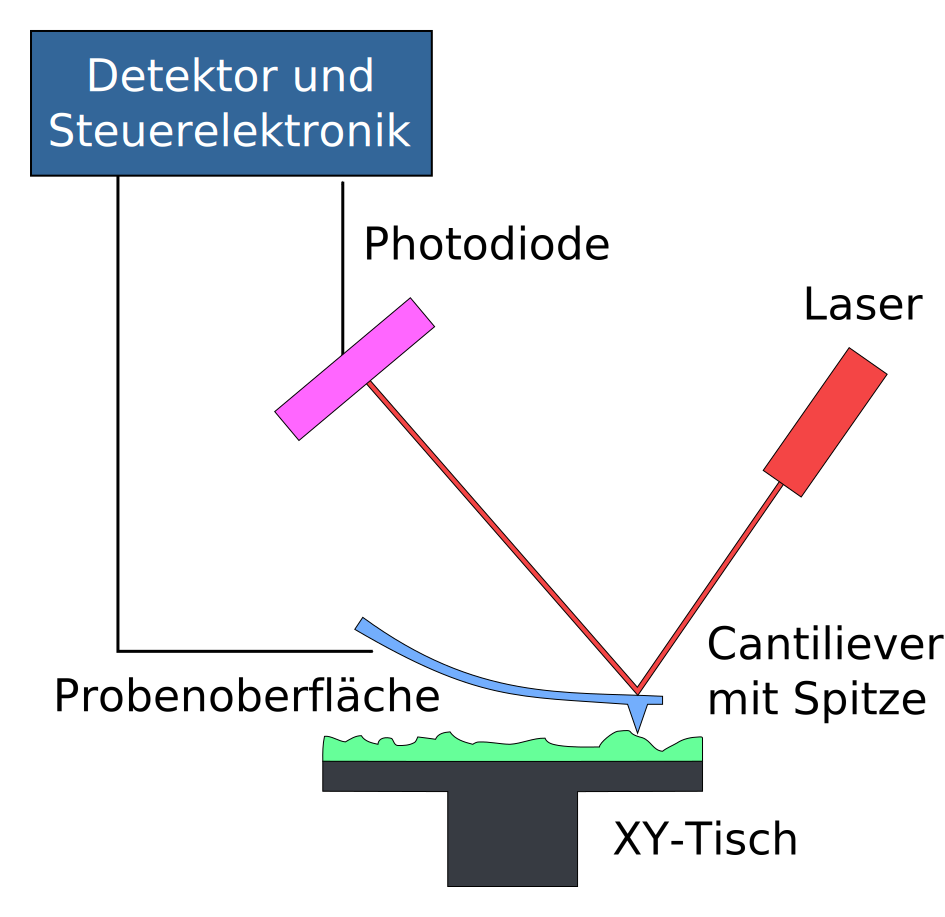
\includegraphics[width=0.4\textwidth]{Atomic_force_microscope_block_diagram_(de).png}
					\caption{Aufbau einer AFM \cite{Wiki:AFM}}
				\end{wrapfigure}

			Bei dieser Messmethode wird mit einem sog. \tilt{Cantilever} (Blattfeder) und einer daran befestigten Nanometer-großen Nadel eine diskretisierte Oberfläche abgerastert. Die Rasterung mit Hilfe von Piezo-Elementen kann hauptsächlich auf 3 Arten der Lagerung von Spitze zur Probe erfolgen: Kontakt, Nicht-Kontakt und intermittierend. Aufgrund der Wechselwirkung (atomare Kräfte, \tilt{atomic forces}) Spitze-Oberfläche biegt sich der feine Cantilever unterschiedlich stark. Diese Verbiegung kann auf verschiedene Weisen - piezo-elektronische Verfahren, optische/interferometrische Messung oder kapazitive Steuerung - gemessen werden, wodurch auf das Profil der Probe geschlossen wird. Bei den erwähnten atomaren Kräften geht es für größere Abstände (einige Mirko-Meter) um die langreichweitigen, anziehenden \tilt{Van-der-Waals-} und Kappillarkräfte. Für Entfernungen Spitze-Oberfläche von wenigen Nano-Metern üben die kurzreichweitigen, abstoßenden Austausch- (auf Grund der Überlappung von Orbitalen der Atome in der Spitze und Oberfläche) und Coulomb-Wechselwirkung einen größeren Einfluss auf die Cantilever-Biegung aus.\\
			Beim Kontakt-Modus der Messung steht die Spitze in direktem, mechanischen Kontakt zur Probe. Die voranging erfahrene Kraft am Cantilever kommt aus der Coulomb-Abstoßung. Einerseits kann man dabei für eine konstante Höhe der Nadel, oder, in Zusammenarbeit mit einem Piezo-Steuerelement, eine konstante Kraft auf diese und somit entsprechende Verbiegung des Cantilevers rastern.\\
			Im Nicht-Kontakt-Modus wird die Feder elektrisch zur Schwingung mit ihrer Resonanz-Frequenz angeregt. Die Frequenz-Antwort des Cantilevers bei der Wechselwirkung mit der Oberfläche kann als Dämpfung aufgefasst werden. Diese Frequenz-Verschiebung Damit gewinnt man Informationen über die Beschaffenheit der Probe.\\
			Während des Intermittierenden Modus oder auch \tilt{tapping mode} wird, ähnlich wie zuvor, die Anregung des Cantilevers nahe seiner Resonanz vorgenommen. Die Regelung des Schwingkreises, die Amplitude der Spitzen-Schwingung konstant zu halten, liefert eine Veränderung des Abstandes und damit Anpassung an die Kraftwechselwirkung mit der Oberfläche. Diese Betriebsart ist ideal für Proben mit empfindlichen Strukturen, die möglicherweise nicht beschädigt werden sollen. Insbesondere liefert der tapping mode die besten Ergebnisse (im Hinblick auf Verfälschung der Messung), da dieser die Kolloide in diesem Versuch nicht verschiebt oder - stellt man sich eine Kugel, welche über eine andere Kugel hinweg läuft (idealisiert) vor, so entsteht ein gewisser Fehler auf Basis ihrer Radien und geometrischen Formen - einen systematischen Fehler mit sich bringt.

				\begin{figure}[t]
					\centering
					\begin{subfigure}{0.48\textwidth}
						\includegraphics[width=\textwidth]{AFM_(used)_cantilever_in_Scanning_Electron_Microscope,_magnification_50000x.png}
						\caption{}
					\end{subfigure}
					\begin{subfigure}{0.48\textwidth}
						\includegraphics[width=\textwidth]{Afm_cd-rom.png}
						\caption{}
					\end{subfigure}
					\caption{\textbf{(a)}: Benutzte AFM-Spitze, Elektronenmikroskop-Aufnahme \textbf{(b)}:AFM-Aufnahme einer CD-ROM \cite{Wiki:AFM}}
				\end{figure}

		\subsection{Röntgenreflektometrie}\label{subsec:röntgen}

				\begin{figure}[t]
					\centering
					\includegraphics[width=0.55\textwidth]{rontgen2.png}
					\caption{Schema der Reflektion von Röntgenstrahlung an einer nicht-glatten Oberfläche \cite{EMAUGreifswaldMIE}}
				\end{figure}

			Die Röntgenflektometrie ist eine analytische, spektroskopische Oberflächenuntersuchung, bei der man sich den Eigenschaften von Röntgenstrahlen und dessen Streuung an dünnen Schichten mit nicht perfekt glatter Struktur zu Nutze macht.\\
			Dabei beobachtet man, die unter einem sehr flachen Einfallswinkel eintreffenden Röntgenstrahlen nach ihrer Reflexion. Dem \tilt{Senllius'schen Brechungsgesetz} zur Folge geht man davon aus, dass das Maximum dessen Intensität beim Einfallswinkel liegt - man verwendet daher ein sog. \tilt{Goniometer} ($2\vartheta$-Anordnung). Weicht die Struktur von der gemachten Forderung ab, so stimmen auch nicht mehr die von den \tilt{Fresnel-Gleichungen} vorhergesagten Intensitäten mit den gemessenen überein. Dies ist insbesondere für genügende Messgenauigkeit immer der Fall.\\
			Mit der Idee, dass in der Röntgenoptik der Brechnungsindex wie \autoref{eq:brechung} geht und das die Reflexion - im speziellen also Transmission, Emission und daraus folgend Absorption - von der elektronischen Struktur der Oberfläche abhängt, ergibt sich grundlegend für das Verhältnis aus gemessener Reflektivität $R$ und \tilt{fresne'lscher} Reflektivität $R\ix{F}$\,:

				\begin{align}
					\frac{R\left(q\ix{z}\right)}{R\ix{F}\left(q\ix{z}\right)}=&\left|\frac{1}{\rho\ix{$\infty$}}\right.\left.\int_{-\infty}^{\infty}\exp\left(\imag q\ix{z}z\right)\frac{\diff \rho\ix{e}}{\diff z}\diff z\right|^2\,\,. \label{eq:edichte}\\
					n=&1-\delta+\imag\beta\approx 1-\frac{\rho\ix{e}r\ix{0}\lambda^2}{2\pi} \label{eq:brechung}
				\end{align}

				\begin{figure}[H]
					\centering
					\includegraphics[width=0.6\textwidth]{rontgenreflekt.png}
					\caption{Reflektion an einer Schicht der Dicke $\Delta$ mit Wellenvektor-Übertrag zwischen A1, A2, A3... \cite{USiegenMIE}}
				\end{figure}

			Hierbei ist $\lambda$ die Röntgenstrahlen-Wellenlänge, $r\ix{0}$ der klassische Elektronenradius, $\rho\ix{e}$ die Elektronendichte der Oberflächenstruktur und $\rho\ix{$\infty$}$ die Dichte im Festkörper.\\
			Der Wellenvektor-Übertrag $q\ix{z}$ von einfallender zu reflektierter Welle steht über die \tilt{Bragg-Reflexion} mit der Schicht- bzw. Gitterdicke des reflektierenden Materials $d$ in Zusammenhang (siehe \autoref{eq:vektoruber}). Dieser Übertrag moduliert bzw. quantifiziert die Reflektivität, weswegen aus dem Abstand zweier Maxima $\alpha\ix{m}$ im Transmissionsspektrum auf die Schicht über \autoref{eq:bragg} geschlossen werden kann.

				\begin{align}
					q\ix{z}=&\frac{4\pi\sin\left(\alpha\right)}{\lambda} \label{eq:vektoruber} \\
					d=&\frac{2\pi}{\Delta q\ix{z}}=\frac{m\lambda}{2\sin\left(\alpha\ix{m}\right)} \label{eq:bragg}
				\end{align}

	\newpage
	\section{Durchführung}

		In Vorbereitung auf die Experimente mit Röntgenreflektometrie, AFM und einer Absorptionsspektroskopie (\tilt{UV-Vis}) galt es, verschieden dichte Monoschichten von Goldpartikeln auf Objekt-Trägern abzulagern. Mit Hilfe von positiv geladenen Substraten  (\tilt{PEI} - Polyelktrolyte), welche die Adsorption der negativ geladenen Goldkolloide auf dem Träger aus einer Suspension ermöglichen, wurden für 45 und $\unit[150]{min}$ eine und für $\unit[90]{min}$ zwei Proben hergestellt. Hierbei handelte es sich um aminoterminierte Silane, welche einerseits kovalent an die Glasoberfläche gebunden wurden.\\
		Die Absorptionsspektroskopie bestand aus der Aufnahme von Spektren der unterschiedlichen Goldschichten in verschiedenen Lösungsmitteln bzw. Reinst-Wasser und Luft. Dabei befanden sich besagte Proben wiederum in Glas- bzw. Plastikküvetten. Eine Einzelmessung bestand aus dem Durchgang eines Referenzstrahls durch die freie Versuchskammer und einem durch die Probe, wobei für beide ein Wellenlängen-Spektrum zwischen $\unit[320-720]{nm}$ durchgestimmt wurde.\\
		Im Vorfeld der Röntgenreflektometrie wurde das Goniometer justiert. Anschließend durchlief die Messung einen Winkelbereich von $\unit[0]{\degree}<\theta<\unit[90]{\degree}$, wobei  letzteres einem senkrechten Ein- und Ausfall der Strahlung entsprach. Eine entsprechende Software berechnete aus dem erhaltenen Intensitätsspektrum den Wellenvektor-Übertrag, welcher für die Berechnung der Schichtdicke genutzt werden kann.\\
		Schließlich galt es, die im \tilt{tapping mode} aufgenommen Höhenprofil-Daten der AFM auszuwerten. Eine Bestimmung eines Einzelteilchen-Radius mittels der vorliegenden Software und einer mittleren Dichte wurde vorgenommen.

	\newpage
	\section{Auswertung}\label{sec:auswertung}

		\subsection{Spektrometrie mit dem \tilt{UV-Vis}}\label{subsec:uvvis}

			\subsection*{Vergleich mit der Theorie}

			Zuerst wurden die theoretischen Rechnung zu den spektroskopischen Größen aus \autoref{subsec:miestreu} durchgeführt. Mit den Daten der AFM über Teilchendichte in der Monoschicht und Partikelradius (siehe \autoref{subsec:auswerafm}) konnte ein Füllfaktor von

				\begin{align}
					f=V\ix{0}N=\frac{4}{3}\pi \overline{R}^3 N= \frac{4\pi}{3}(\unit[15]{nm})^3\cdot\frac{54,5}{(\unit[500]{nm})^2\cdot\overline{R}}=0,2198(03)
				\end{align}

			berechnet werden. Mit den Kenntnissen über die Wertepaare Photonenenergie - $n(\lambda)$ bzw. $\kappa(\lambda)$ und diesem Füllfaktor bzw. den angegebenen Dielektrizitätskonstanten $\varepsilon\ix{m}$ der umgebenden Medien konnten die erwähnten Kalkulationen durchgeführt werden (siehe \autoref{sec:anhang} für den entsprechenden Quellcode).\\
			Zuerst galt es die Imaginär- und Realteile der einfachen Dielektrizitätskonstanten $\varepsilon(\lambda)$, des Maxwell-Garnett-Koeffizienten nach \autoref{eq:maxwellgarnett} und daraus folgend der effektiven Größe $\varepsilon\ix{eff}$ aus \autoref{eq:effektdielektr} darzustellen. Die Ergebnisse repräsentieren \autoref{img:epsilon}, \autoref{img:kappaun} sowie \autoref{img:epsilon_eff}. Die Darstellung erfolgte über einen Wellenlängenbereich von $\unit[400]{nm}<\lambda<\unit[720]{nm}$.

				\begin{figure}[H]
					\includegraphics[width=0.9\textwidth]{epsilon_uber_lambda.png}
					\caption{Dielektrizitätskonstante für Gold-Kolloide in einer wässrigen Lösung mit $\varepsilon\ix{m}\approx1,77$, Imaginär- und Realteil aufgetrennt (theoretisch).}
					\label{img:epsilon}
				\end{figure}

				\begin{figure}[H]
					\includegraphics[width=\textwidth]{kappaun_uber_lambda.png}
					\caption{Imaginär- und Realteil des Brechnungsindex $\tilde{n}(\lambda)=\sqrt{\varepsilon(\lambda)}$ in Form von $n(\lambda)$,$\kappa(\lambda)$ (theoretisch).}
					\label{img:kappaun}
				\end{figure}

				\begin{figure}[H]
					\includegraphics[width=\textwidth]{epsilon_eff_uber_lambda.png}
					\caption{Effektive Dielektrizitätskonstante für $f=0,2198$ unter Rücksichtnahme auf eine endliche Teilchendichte der Kolloide und deren Wechselwirkung (theoretisch).}
					\label{img:epsilon_eff}
				\end{figure}

			Der gemachten Rechnungen schließt sich der Vergleich von Theorie und Messung an. Geeigneter Weise wurde eine Lösung von kolloidalem Gold der Dichte $\unit[2,4]{\frac{nmol}{L}}$ spektroskopisch untersucht. In \autoref{img:vergleich} sind Extinktions-Koeffizienten-Verläufe für die Berechnung nach \autoref{eq:extinkt-intens} und der Differenz aus $Au$-Suspension und Wasser zu sehen.  Die Darstellung erfolgte über ein Spektrum von $\unit[400]{nm}<\lambda<\unit[720]{nm}$. Hierbei wurde die Küvettenlänge (das heißt die Weite des Durchgangsmediums) auf $D=\unit[1]{cm}$ angesetzt. Auffällig ist die Verschiebung des Wellenlängen-abhängigen Maximums. Für $\gamma\ix{theo}$ liegt dieses bei $\gamma\ix{max,theo}\approx\unit[3,77(49)]{m^{-1}}$ bei $\lambda\ix{max,theo}\approx\unit[537,7(19)]{nm}$, aus der Messung folgt $\gamma\ix{Mess,theo}\approx\unit[4,39(35)]{m^{-1}}$ um $\lambda\ix{max,Mess}\approx\unit[400,8(59)]{nm}$. Des weiteren sind die Ausprägungen der Maxima und Abszissen-Abschnitte beider Graphen unterschiedlich.

				\begin{figure}[H]
					\centering
					\includegraphics[width=\textwidth]{theo_gamma_abs_goldloes.png}
					\caption{Vergleich von Theorie und Messung der Extinktionskoeffizienten für eine Kolloid-Lösung von Gold als Funktion der Wellelänge.}
					\label{img:vergleich}
				\end{figure}

			\subsection*{Spektren von Gold-Monoschichten in Luft und Lösungen}

			Im Folgenden werden die Spektren und insbesondere die Extinktionskoeffizienten der Gold-Adsoprtionen in verschiedenen Umgebungen/Lösungsmitteln präsentiert und mit den theoretischen Zusammenhängen verglichen.\\
			Beginnend mit den Messungen in Luft, stellt \autoref{img:luft} die Ergebnisse dar. Lediglich die Zeit, welche die PEI-beschichteten Proben in der Gold-Lösung verbracht haben (45 und 90 Minuten), unterscheidet sie. \autoref{tab:luft} listet die Daten der Maxima auf.\\
			Obwohl die erhaltenen Punkte der Extrema sich sehr ähneln, sehen die Spektren doch stark unterschiedlich aus. Der Graph zur 150-minütigen Probe gleicht in Näherung der Theorie bzw. den bisher betrachteten Ergebnisse, wohingegen die Messung der früheren Ablagerung einen sehr unterschiedlichen Absorptions-Verlauf ergibt. Für niedrigere Wellenlängen ist der Anstieg ähnlich - die verwendeten Küvetten waren gleich und deswegen ist die Auslöschung des Nah-UV- bzw. UV-Lichts vergleichbar. Ein angedeutetes Minimum vor dem Maximum tritt für die 45-minütige Probe viel stärker hervor, als es das für die andere tut. Ebenso ist schemenhaft ein Peak nahe des, im Spektrum der $\unit[150]{min}$-Probe klar hervortretenden Maximums zu sehen. Dieser geht jedoch für größere Wellenlängen im restlichen Verlauf unter.

			\begin{table}[H]
				\centering
				\begin{tabular}{c|c|c|}
					Zeit zur Adsorption & $\gamma\ix{max}/\unit{m^{-1}}$ & $\lambda\ix{max}/\unit{nm}$ \\ 
					\hline\hline $\unit[45]{min}$ & 0,940(73) & 399,9(70)  \\
					\hline $\unit[150]{min}$ & 0,446(22) & 400,8(80)
				\end{tabular} 
			\caption{Daten der Maxima zu \autoref{img:luft}. Maximaler Extinktionskoeffizient mit seiner Resonanz-Wellenlänge.}
			\label{tab:luft}
			\end{table}

				\begin{figure}[H]
					\centering
					\includegraphics[width=\textwidth]{absorp_spektren_luft.png}
					\caption{Vergleich des gemessenen Extinktions-Spektrum in Luft zwischen 2 unterschiedlich lange behandelten Proben (unterschiedliche Monoschichten-Dichten).}
					\label{img:luft}
				\end{figure}

			Abschließend betrachtet und wertet man die Extinktions-Koeffizienten für Gold-Adsorptionen über $\unit[90]{min}$ in den Lösungsmitteln Propandiol, Brombenzol, Nitromethan und Toluol aus. Die \autoref{tab:loesungen} zeigt wie im Vorherigen die Zusammenhänge der Extrema, welche in \autoref{img:loesgemess} der gemessenen und \autoref{img:loestheo} der theoretischen Spektren zu erkennen sind.\\
			Der gravierende Unterschied zwischen den Werten in der Tabelle kann u.a. auf den Einfluss der Oberfläche, auf welcher sich die Monoschicht befindet, begründet werden. Die angeführte Streutheorie aus \autoref{subsec:miestreu} geht auf 2-D-System zurück. Dies ist offensichtlich eine große Vernachlässigung der elektronischen Wechselwirkung mit dem PEI oder der Glasplatte. Insbesondere ist der Einfluss des umgebenden Mediums nur auf die Höhe der Extinktions-Resonanz beschränkt, verändert also nicht die Position (Wellenlänge) des Verlaufs. Die Spektrometrischen Eigenschaften der Gold-Monoschicht allgemeine werden nicht beeinflusst.

				\begin{table}[H]
					\centering
					\begin{tabular}{c|c|c|c|c|c}
						Lösungsmittel & $\varepsilon\ix{m}$ & $\gamma\ix{max,mess}/\unit{m^{-1}}$ & $\lambda\ix{max,mess}/\unit{nm}$ & $\gamma\ix{max,theo}/\unit{m^{-1}}$ & $\lambda\ix{max,theo}/\unit{nm}$ \\ 
						\hline\hline Wasser & 1,77 & 1,2599 &  401,84 & 0,0377 & 537,719 \\
						\hline Brombenzol & 1,5602 & 3,666 & 401,849 & 0,0354 & 537,719 \\
						\hline Propandiol & 1,43 & 1,30455 & 401,84 & 0,0339 & 537,719 \\
						\hline Toluol & 1,496 & 0,968 & 400,77 & 0,0347 & 537,719 \\
						\hline Nitromethan & 1,3818 & 12,776 & 401,62 & 0,0335 & 537,719
					\end{tabular} 
					\caption{Daten der Maxima - sowohl theoretisch als auch gemessen - für die angegebenen Lösungsmittel.}
					\label{tab:loesungen}
				\end{table}
	
				\begin{figure}[H]
					\centering
					\includegraphics[width=\textwidth]{absorp_spektren_loesungen.png}
					\caption{Extinktions-Spektren der $\unit[90]{min}$-Adsorption in verschiedenene Lösungsmitteln (siehe \autoref{tab:loesungen}).}
					\label{img:loesgemess}
				\end{figure}
	
				\begin{figure}[H]
					\centering
					\includegraphics[width=\textwidth]{theoret_maxima_loesung.png}
					\caption{Extinktions-Spektren der theoretischen Absorption verschiedenene Lösungsmittel (siehe \autoref{tab:loesungen}).}
					\label{img:loestheo}
				\end{figure}

		\subsection{AFM und Röntgenreflexion - Größenbestimmungen}\label{subsec:auswerafm}

			Zuerst wird die Messung mit der Röntgenreflexion ausgewertet.\\
			Die \autoref{img:rontgen} zeigt das Spektrum $R(q\ix{z})/R\ix{F}(q\ix{z})$ in Abhängigkeit des Wellenvektor-Übertrags $q\ix{z}$. Der Graph erlaubt nur die Entnahm eines $\Delta q\ix{z}$ zwischen 2 Maxima des Resonanzverlaufs nach \autoref{eq:vektoruber}. Mit eine $\Delta q\ix{z}= |0.3307-0.4339|\cdot\unit[\tenpo{9}]{nm^{-1}}$ ergibt sich nach \autoref{eq:vektoruber} die Schichtdicke in \autoref{eq:rontgendick}. Dieses Ergebnis ist besonders auffällig, da im Vergleich zu denen aus \autoref{tab:radien} hier in etwa der doppelte Wert vorliegt.

				\begin{align}
					d=\frac{\pi}{\Delta q\ix{z}}=\unit[30,044(17)]{nm} \,\,.
				\end{align}

				\begin{figure}[H]
					\centering
					\includegraphics[width=\textwidth]{rontgenreflexion.png}
					\caption{Quotient aus gemessener Relektivität zu fresnel'scher Reflektivität über dem Wellenvektor-Übertrag.  Verwendet wurde die Probe mit 90-minütiger Adsorption.}
					\label{img:rontgen}
				\end{figure}

			Abschließend gilt es, die Messungen mit dem AFM zu betrachten. Die erhaltenen Höhen-Profile zeigt \autoref{img:afm}, einmal für einen Ausschnitt von $\unit[1]{\mu m^2}$ und für $\unit[25000]{nm^2}$. Mit Hilfe der vorhandenen Software war es möglich, die Teilchenhöhe, dh. $2\cdot R$ zu bestimmen. Die erhaltenen Wert enthält \autoref{tab:radien}. Darauf ergibt sich ein durchschnittlicher Kolloid-Radius von $\unit[15.5297]{nm}$. Nach der Auswertung - e.g. Auszählen der "`echten"'  Partikel der Schicht - von allen 4 Quadranten im linken Teil von \autoref{img:afm}, erhält man eine mittlere Teilchendichte von 54,5 Kolloiden je Monoschicht und $\unit[25000]{nm^2}$. Diese Daten konnten damit in den Berechnungen für die UV-Vis-Untersuchungen verwendet werden.

			\begin{table}[H]
				\centering
				\begin{tabular}{|c||c|c|c|c|c}
					Partikel-Nr. & 1 & 2 & 3 & 4 & 5  \\ 
					\hline  Radius R/$\unit{nm}$ & 16,173 & 18,584 & 15,472 & 14,281 & 15,106 
				\end{tabular}
				\begin{tabular}{c|c|c|c|c|c}
					6 & 7 & 8 & 9 & 10 & $\overline{R}$ \\
					\hline 14,191 & 13,824 & 14,038 & 16,784 & 16,844 & 15,5297
				\end{tabular}
				\caption{Ausgemessene Radien an den Aufnahmen in \autoref{img:afm} und der mittlere Teilchenradius in der Monoschicht $\overline{R}$.}
				\label{tab:radien}
			\end{table}

			\begin{figure}[H]
				\centering
				\includegraphics[width=\textwidth]{au90minbeide.jpg}
				\caption{Aufnahmen des Höhen-Profils der Gold-Monoschicht einer 90-minütigen Adsorption. Links ist ein $500\times500\,\unit{nm^2}$-Abschnitt zu sehen, rechts der dazugehörige $\unit[1]{\mu m^2}$-Bereich.}
				\label{img:afm}
			\end{figure}

		\subsection{Fazit}

			Der Versuch zur Mie-Streuung gewährte viele Eindrücke in die Oberflächen- und Nano-Physik. Insbesondere die beeindruckende Messauflösung von rein mechanischen Verfahren wie der AFM erzielte gute Ergebnisse. Wiederum war der Erfolg mit Röntgenreflexion - e.g. der Verlauf des Spektrums - und dem UV-Vis ernüchternd. Entgegen der Voraussagen aus Theorie , welche u.a. direkt zum Vergleich gesetzt wurde, konnten einige Eigenschaften nicht nachvollzogen werden. Jedoch sind generell die Annahmen bestätigt worden - speziell im Hinblick auf die allgemeine Form der Absorptions-Spektren.\\
			Fehlerquellen wie die, in der Theorie gemachte Vernachlässigung der dritten Dimension in der Beschreibung von Absorption und Extinktion einer Gold-Monoschicht auf einem Glas-Träger und die nicht-ideale Adsorption auf den Platten (vor allem mit Einbau von deformierten Fehlstellen, e.g. Staub) verhinderten bessere Ergebnisse.

	\newpage
	\section{Anhang}\label{sec:anhang}

		Hier folgt auf den nächsten Seiten ebenso der Quellcode des verwendeten Programms zur Berechnung der Real- und Imaginärteile der Koeffizienten für die Spektroskopie sowie die gemachte Auswertung.

		\bibliography{all.bib}
		\bibliographystyle{unsrt}

	\newpage


	\lstset{
		flexiblecolumns=true,
		numbers=left
	}

\begin{lstlisting}
function [] = mie_spektren_rechner

clear all;

%Wellenlaenge (aus Energie der Photonen ueber lambda=h*c/E) und Vektor
lambda=(1239.841974)./[1.2:0.2:2.0 2.1 2.2 2.4 2.5 2.6 2.7 2.8 2.9 3.0 3.1]';
lambi=[min(lambda):0.01:max(lambda)]';

%Werte von n und Interpolation dazwischen
n=[0.1 0.08 0.08 0.09 0.13 0.18 0.24 0.5 0.82 1.24 1.43 1.46 1.5 1.54 1.54]';
ni=interp1(lambda,n,lambi,'spline');

%Werte von k und Interpolation dazwischen
k=[6.54 5.44 4.56 3.82 3.16 2.84 2.54 1.86 1.59 1.54 1.72 1.77 1.79 1.8 1.81]';
ki=interp1(lambda,k,lambi,'spline');

%e_m fuer waessrige Loesung mit Glasplatte, f=0.2
e_m=1.77;
f=0.219803437590171;

figure;
hold all;
grid on;
title('Real- und Imaginaerteil der Brechnung');
xlabel('\lambda/nm');
ylabel('\kappa,n');
plot(lambi,ki,'LineWidth',2.5);
plot(lambi,ni,'LineWidth',2.5);
legend('\kappa','n');
set(gca, 'FontSize', 20);
axis([400 720 0 6.5]);
hold off;

%Berechnen des Imaginaer- und Realteils von epsilon
e_re=-(ki.^2-ni.^2);
e_im=sqrt(4*(ni.^2-e_re/2).^2-e_re.^2);

figure;
hold all;
grid on;
title('Real- und Imaginaerteil der dielektrischen Funktion');
xlabel('\lambda/nm');
ylabel('\epsilon_{Re/Im}');
plot(lambi,e_re,'LineWidth',2.5);
plot(lambi,e_im,'LineWidth',2.5);
legend('\epsilon_{Re}','\epsilon_{Im}');
set(gca, 'FontSize', 20);
axis([400 720 min(e_re)-0.1*min(e_re) max(e_im)+0.1*max(e_im)]);
hold off;

%Lambda(Maxwell-Garnett) in imag und real aufteilen
L_re=(e_re.^2+e_im.^2-2.*e_m.^2+e_re.*e_m)./((e_re+2*e_m).^2+e_im.^2);
L_im=(3*e_im.*e_m)./((e_re+2*e_m).^2+e_im.^2);

%Real und Imag von effektiver dielektrischen Funktion
e_effre=e_m*(L_re*f+1-2*f^2.*L_re.^2-2*f^2.*L_im.^2)./((1-L_re*f).^2+L_im.^2*f^2);
e_effim=e_m*(3*f.*L_im)./((1-L_re*f).^2+L_im.^2*f^2);

figure;
hold all;
grid on;
title('Real- und Imaginaerteil der effektiven dielektrischen Funktion');
xlabel('\lambda/nm');
ylabel('\epsilon_{eff,Re/Im}');
plot(lambi,e_effre,'LineWidth',2.5);
plot(lambi,e_effim,'LineWidth',2.5);
legend('\epsilon_{eff,Re}','\epsilon_{eff,Im}');
set(gca, 'FontSize', 20);
axis([400 720 min(e_effim) max(e_effre)]);
hold off;

kap=sqrt(-e_effre./2+sqrt(e_effre.^2+e_effim.^2)./(2));

figure;
hold on;
grid on;
title('exp(-\kappa)');
plot(lambi, exp(-kap),'LineWidth',2.5);
legend('exp(\kappa)');
xlabel('\kappa');
ylabel('exp(-\kappa)');
set(gca, 'FontSize', 20);
axis([400 1000 min(exp(-kap))-0.1 max(exp(-kap))+0.1]);
hold off;

figure;
hold on;
grid on;
xlabel('\lambda/nm');
ylabel('\kappa');
plot(lambi, kap,'LineWidth',2.5);
legend('\kappa');
set(gca, 'FontSize', 20);
axis([400 1000 min(kap)-0.1*min(kap) max(kap)+0.1*max(kap)]);
hold off;

gamma =4*pi*kap./lambi;

load('C:\Users\Philipp Hacker\Desktop\Uni\git\fpraktikum_mit_alex\Mie-Streuung\Peiauair150minedit.txt');
load('C:\Users\Philipp Hacker\Desktop\Uni\git\fpraktikum_mit_alex\Mie-Streuung\Peiaubr90minedit.txt');
load('C:\Users\Philipp Hacker\Desktop\Uni\git\fpraktikum_mit_alex\Mie-Streuung\Peiauh2o90minedit.txt');
load('C:\Users\Philipp Hacker\Desktop\Uni\git\fpraktikum_mit_alex\Mie-Streuung\Peiauni90minedit.txt');
load('C:\Users\Philipp Hacker\Desktop\Uni\git\fpraktikum_mit_alex\Mie-Streuung\Peiaupro90minedit.txt');
load('C:\Users\Philipp Hacker\Desktop\Uni\git\fpraktikum_mit_alex\Mie-Streuung\Peiautol90minedit.txt');
load('C:\Users\Philipp Hacker\Desktop\Uni\git\fpraktikum_mit_alex\Mie-Streuung\PEIBRedit.txt');
load('C:\Users\Philipp Hacker\Desktop\Uni\git\fpraktikum_mit_alex\Mie-Streuung\PEIedit.txt');
load('C:\Users\Philipp Hacker\Desktop\Uni\git\fpraktikum_mit_alex\Mie-Streuung\PEIH2Oedit.txt');
load('C:\Users\Philipp Hacker\Desktop\Uni\git\fpraktikum_mit_alex\Mie-Streuung\PEINIedit.txt');
load('C:\Users\Philipp Hacker\Desktop\Uni\git\fpraktikum_mit_alex\Mie-Streuung\PEIPROedit.txt');
load('C:\Users\Philipp Hacker\Desktop\Uni\git\fpraktikum_mit_alex\Mie-Streuung\PEITOLedit.txt');
load('C:\Users\Philipp Hacker\Desktop\Uni\git\fpraktikum_mit_alex\Mie-Streuung\AULSGedit.txt');
load('C:\Users\Philipp Hacker\Desktop\Uni\git\fpraktikum_mit_alex\Mie-Streuung\Peiauair45minedit.txt');
load('C:\Users\Philipp Hacker\Desktop\Uni\git\fpraktikum_mit_alex\Mie-Streuung\H2Oedit.txt');

figure;
hold on;
grid on;
fprintf(1,'Maxima des Theorie-Vergleichs\n');
plot(lambi,100*gamma,'LineWidth',2.5);

[gamma_m,x] = max(100*gamma);
lamb_max = lambi(x);
fprintf(1,'Gamma -- e_m = 1.77, gamma_max = %d m^{-1}, lambda_max = %d nm\n', gamma_m, lamb_max);

plot(H2Oedit(:,1),log(1/min((10.^(AULSGedit(:,2))-10.^(H2Oedit(:,2))))*(10.^(AULSGedit(:,2))-10.^(H2Oedit(:,2)))),'LineWidth',2.5);

[gamma_m,x] = max(log(1/min((10.^(AULSGedit(:,2))-10.^(H2Oedit(:,2))))*(10.^(AULSGedit(:,2))-10.^(H2Oedit(:,2)))));
lamb_max = lambi(x);
fprintf(1,'Au-Lsg -- e_m = 1.77, gamma_max = %d m^{-1}, lambda_max = %d nm\n', gamma_m, lamb_max);

axis([400 720 0 4.5]);
xlabel('\lambda/nm');
ylabel('\gamma in m^{-1}, Absorptionskoeff.');
legend('\gamma_{theo}','Abs(Au-Loes.)-Abs(H_{2}O)');
set(gca, 'FontSize', 20);
hold off;

figure;
hold on;
grid on;
%plot(lambi,100*gamma,'LineWidth',2.5);
fprintf(1,'gemessene Maxima\n');
plot(H2Oedit(:,1),log(1/min(10.^(Peiauh2o90minedit(:,2))-10.^(PEIH2Oedit(:,2)))*(10.^(Peiauh2o90minedit(:,2))-10.^(PEIH2Oedit(:,2)))),'LineWidth',2.5);

[gamma_m,x] = max(log(1/min(10.^(Peiauh2o90minedit(:,2))-10.^(PEIH2Oedit(:,2)))*(10.^(Peiauh2o90minedit(:,2))-10.^(PEIH2Oedit(:,2)))));
lamb_max = lambi(x);
fprintf(1,'PEI_au, H2O. 90min. -- e_m = 1.77, gamma_max = %d m^{-1}, lambda_max = %d nm\n', gamma_m, lamb_max);

plot(H2Oedit(:,1),log(1/min((10.^(Peiautol90minedit(:,2))-10.^(PEITOLedit(:,2))))*(10.^(Peiautol90minedit(:,2))-10.^(PEITOLedit(:,2)))),'LineWidth',2.5);

[gamma_m,x] = max(log(1/min((10.^(Peiautol90minedit(:,2))-10.^(PEITOLedit(:,2))))*(10.^(Peiautol90minedit(:,2))-10.^(PEITOLedit(:,2)))));
lamb_max = lambi(x);
fprintf(1,'PEI_au,Toluol. 90min. -- e_m = 1.496, gamma_max = %d m^{-1}, lambda_max = %d nm\n', gamma_m, lamb_max);

plot(H2Oedit(:,1),log(1/min((10.^(Peiaubr90minedit(:,2))-10.^(PEIBRedit(:,2))))*(10.^(Peiaubr90minedit(:,2))-10.^(PEIBRedit(:,2)))),'LineWidth',2.5);

[gamma_m,x] = max(log(1/min((10.^(Peiaubr90minedit(:,2))-10.^(PEIBRedit(:,2))))*(10.^(Peiaubr90minedit(:,2))-10.^(PEIBRedit(:,2)))));
lamb_max = lambi(x);
fprintf(1,'PEI_au,Brombenzol. 90min. -- e_m = 1.5602, gamma_max = %d m^{-1}, lambda_max = %d nm\n', gamma_m, lamb_max);

plot(H2Oedit(1:168,1),log(1/min((10.^(Peiauni90minedit(1:168,2))-10.^(PEINIedit(1:168,2))))*(10.^(Peiauni90minedit(1:168,2))-10.^(PEINIedit(1:168,2)))),'LineWidth',2.5);

[gamma_m,x] = max(log(1/min((10.^(Peiauni90minedit(1:168,2))-10.^(PEINIedit(1:168,2))))*(10.^(Peiauni90minedit(1:168,2))-10.^(PEINIedit(1:168,2)))));
lamb_max = lambi(x);
fprintf(1,'PEI_au,Nitromethan. 90min. -- e_m = 1.3818, gamma_max = %d m^{-1}, lambda_max = %d nm\n', gamma_m, lamb_max);

plot(H2Oedit(:,1),log(1/min((10.^(Peiaupro90minedit(:,2))-10.^(PEIPROedit(:,2))))*(10.^(Peiaupro90minedit(:,2))-10.^(PEIPROedit(:,2)))),'LineWidth',2.5);

[gamma_m,x] = max(log(1/min((10.^(Peiaupro90minedit(:,2))-10.^(PEIPROedit(:,2))))*(10.^(Peiaupro90minedit(:,2))-10.^(PEIPROedit(:,2)))));
lamb_max = lambi(x);
fprintf(1,'PEI_au, Propandiol 90min. -- e_m = 1.43, gamma_max = %d m^{-1}, lambda_max = %d nm\n', gamma_m, lamb_max);

xlabel('\lambda/nm');
ylabel('\gamma in m^{-1}');
axis([400 700 0 1]);
legend('Abs(PEI-Au, 90 min., H_{2}O)-Abs(PEI, H_{2}O)','Abs(PEI-Au, 90 min., Toluol)-Abs(PEI, Toluol)','Abs(PEI-Au, 90 min., Bromb.)-Abs(PEI, Bromb.)','Abs(PEI-Au, 90 min., Nitr.)-Abs(PEI, Nitr.)','Abs(PEI-Au, 90 min., Propandiol)-Abs(PEI, Prop.)');
set(gca, 'FontSize', 20);
hold off;

figure;
hold on;
grid on;
fprintf(1,'Maxima aus Luft\n');

plot(H2Oedit(:,1),log(1/min((10.^(Peiauair150minedit(:,2))-10.^(PEIedit(:,2))))*(10.^(Peiauair150minedit(:,2))-10.^(PEIedit(:,2)))),'LineWidth',2.5);

[gamma_m,x] = max(log(1/min((10.^(Peiauair150minedit(1:126,2))-10.^(PEIedit(1:126,2))))*(10.^(Peiauair150minedit(1:126,2))-10.^(PEIedit(1:126,2)))));
lamb_max = lambi(x);
fprintf(1,'PEI Au Luft 150min. -- e_m = 1, gamma_max = %d m^{-1}, lambda_max = %d nm\n', gamma_m, lamb_max);

plot(H2Oedit(:,1),log(1/min((10.^(Peiauair45minedit(:,2))-10.^(PEIedit(:,2))))*(10.^(Peiauair45minedit(:,2))-10.^(PEIedit(:,2)))),'LineWidth',2.5);

[gamma_m,x] = max(log(1/min((10.^(Peiauair45minedit(1:126,2))-10.^(PEIedit(1:126,2))))*(10.^(Peiauair45minedit(1:126,2))-10.^(PEIedit(1:126,2)))));
lamb_max = lambi(x);
fprintf(1,'PEI Au Luft 45min. -- e_m = 1, gamma_max = %d m^{-1}, lambda_max = %d nm\n', gamma_m, lamb_max);

xlabel('\lambda/nm');
ylabel('\gamma in m^{-1}');
axis([320 700 0 1]);
legend('Abs(PEI-Au, 150 min., Luft)-Abs(PEI, Luft)','Abs(PEI-Au, 45 min., Luft)-Abs(PEI, Luft)');
set(gca, 'FontSize', 20);
hold off;

figure;
hold on;
grid on;
set(gca,'FontSize',20);
xlabel('\lambda');
ylabel('\gamma(\lambda) in m^{-1}')
fprintf(1,'Theoretische Werte\n');
for e_m = [1.77 1.3818 1.43 1.496 1.5602];
e_effre=e_m*(L_re*f+1-2*f^2.*L_re.^2-2*f^2.*L_im.^2)./((1-L_re*f).^2+L_im.^2*f^2);
e_effim=e_m*(3*f.*L_im)./((1-L_re*f).^2+L_im.^2*f^2);
kap=sqrt(-e_effre./2+sqrt(e_effre.^2+e_effim.^2)./(2));
gamma =4*pi*kap./lambi;
plot(lambi,100*gamma,'LineWidth',2.5);
[gam_max,x] = max(gamma);
lam_max = lambi(x);
fprintf(1,'e_m = %d -- gamma_max = %d 1/m, lambda_max = %d nm\n', e_m, gam_max, lam_max); 
end;
legend('\epsilon_{m}=1.77, Wasser','\epsilon_{m}=1.3818, Nitromethan','\epsilon_{m}=1.5602, Brombenzol','\epsilon_{m}=1.496, Toluol','\epsilon_{m}=1.43, Propandiol');
axis([528 546 2.8 3.8]);
hold off;

load('xray150.DAT');

figure;
hold on;
grid on;
set(gca,'FontSize',20);
plot(xray150(:,1)*10,xray150(:,2),'LineWidth',2.5);
axis([0 1.2 0 max(xray150(:,2))]);
legend('Roentgenreflektometrie-Daten');
xlabel('q_{z}/nm^{-1}');
ylabel('Intensitaet, a.u.');
hold off;

clear all;

end
\end{lstlisting}

\end{document}